\documentclass[11pt]{article}
\usepackage[letterpaper,margin=1in]{geometry}
\usepackage{graphicx}
\usepackage{booktabs}
\usepackage[hidelinks]{hyperref}
\usepackage{setspace}
\setlength{\parindent}{0pt}
\setlength{\parskip}{0.6em}

\title{\Large\bfseries Supplementary Material}
\author{The Non-Canonical Frontier in Peptide-MHC-I Binding Prediction: A Benchmark-Hygiene Case Study}
\date{}

\begin{document}
\maketitle

\section*{Supplementary Note S --- Molecular Dynamics of the K-E63 Salt Bridge}

This note reports the molecular-dynamics (MD) analysis referenced in the main text
(\S 2.4), which is deliberately excluded from the primary structural argument and
presented here for completeness.

\subsection*{S.1 Methods}
The KRAS G12V neoepitope YKLVVVGAV was modelled into the HLA-A*02:01 peptide-binding
groove using the 1DUZ template (template peptide LLFGYPVYV replaced in silico). The
complex was solvated and equilibrated, then simulated for 100 ns with OpenMM 8.5.2 and
the amber14 force field. Three independent replicas (seeds 42 and 99) were run to assess
convergence. MM-GBSA binding energies were computed over the final 50 ns (200 frames).

\subsection*{S.2 Results}
\textbf{System stability.} The complex remained stable over 100 ns: the MHC $\alpha$-chain,
$\beta$2-microglobulin, and peptide backbone RMSDs converged to 0.15, 0.09, and 0.07 \AA{},
respectively (Fig.~S-MD2). Whole-complex backbone RMSD reached 6.1 \AA{}, reflecting
flexible regions outside the peptide-binding groove.

\textbf{The K-E63 salt bridge is transient, not persistent.} The P2-Lys--Glu63 minimum
distance fluctuated between 3.6 and 5.9 \AA{} across the three replicas (mean $\approx$ 4.1 \AA{}),
with transient close contacts ($<$ 3 \AA{}) in $\sim$14\% of frames in the primary trajectory
(Fig.~S-MD3; Fig.~S-MD1). The salt bridge therefore forms intermittently but does not
persist as a stable interaction over the simulated timescale.

\textbf{Binding energy.} MM-GBSA over the final 50 ns gave $\Delta G = -19.6 \pm 46.3$ kcal/mol
(mean $\pm$ SD, n = 200), dominated by gas-phase electrostatics ($\Delta E = -19.5$ kcal/mol) with a
negligible solvation term. The large variance precludes a precise binding estimate
(Fig.~S-MD4).

\textbf{Hydrogen bonding.} 3,574 unique hydrogen bonds were observed across the trajectory,
with 14 persistent pairs (occupancy $>$ 30\%).

\subsection*{S.3 Interpretation}
The MD is consistent with the conservative framing in the main text (\S 3.5): a charged
P2-Lys can transiently reach Glu63, but the K-E63 salt bridge is not a stable, persistent
interaction over the simulated timescale. These data support treating the salt-bridge
hypothesis as qualitative, pending a more rigorous free-energy calculation (e.g.,
alchemical transformation or umbrella sampling) and experimental validation (e.g., X-ray
crystallography or cryo-EM of the YKLVVVGAV--HLA-A*02:01 complex).

\newpage
\section*{Supplementary Tables --- Findings Summary}
All numbers are validated, cross-predictor, seed-robust, temporal-holdout-checked.

\subsection*{Table S1. Predictor comparison --- canonical vs Type B sensitivity (pooled)}
\begin{table}[h]
\centering
\begin{tabular}{@{}lccc@{}}
\toprule
Predictor class & Canonical sens & Type B (non-canonical) sens & n \\
\midrule
Deep FFN (sequence) & 0.979 & 0.607 & 14,488 \\
MHCflurry (sequence) & 0.986 & 0.668 & 14,488 \\
MUNIS (structure) & 0.950 & 0.647 & 6,224 \\
Takeaway & $\sim$0.98 solved & $\sim$0.65 plateau (all classes) & \\
\bottomrule
\end{tabular}
\end{table}

\subsection*{Table S2. Pan16 --- 15-allele panel, per-allele non-canonical sensitivity}
\begin{table}[h]
\centering
\begin{tabular}{@{}lclc@{}}
\toprule
Allele & sens@0.95 & Allele & sens@0.95 \\
\midrule
HLA-A*02:01 & 0.880 & HLA-B*08:01 & 0.880 \\
HLA-A*01:01 & 0.800 & HLA-B*15:01 & 0.960 \\
HLA-A*03:01 & \textbf{1.000} & HLA-B*27:05 & 0.080 \\
HLA-B*07:02 & 0.640 & HLA-B*35:01 & 0.840 \\
HLA-B*44:03 & \textbf{1.000} & HLA-B*40:01 & \textbf{1.000} \\
HLA-A*11:01 & \textbf{1.000} & HLA-B*49:01 & \textbf{1.000} \\
HLA-A*24:02 & 0.760 & HLA-B*51:01 & 0.520 \\
 &  & HLA-B*57:01 & 0.920 \\
POOLED (15 alleles) & \textbf{0.819} (307/375) &  &  \\
\bottomrule
\end{tabular}
\end{table}

Weak tail = thin-training alleles (B*27:05 n=150, B*51:01 n=1,665) --- data scarcity, not architecture.

\subsection*{Table S3. Temporal holdout --- generalization to post-2022 epitopes}
\begin{table}[h]
\centering
\begin{tabular}{@{}lccc@{}}
\toprule
Allele & pre-2021 sens@0.95 & post-2022 sens@0.95 & Delta \\
\midrule
HLA-A*02:01 & 0.879 (n=2704) & 0.824 (n=1151) & $-0.055$ \\
HLA-A*03:01 & 0.905 (n=1744) & 0.936 (n=803) & \textbf{+0.031} \\
HLA-B*07:02 & 0.898 (n=2315) & 0.973 (n=865) & \textbf{+0.075} \\
\bottomrule
\end{tabular}
\end{table}

Post-2022 epitopes were published after MHCflurry's training cutoff (unseen by the
labeler). Preserved/improved sensitivity = NOT overfit to the IEDB era.

\subsection*{Table S4. P2 virtual mutagenesis --- sidechain reach to Glu63}
\begin{table}[h]
\centering
\begin{tabular}{@{}lccc@{}}
\toprule
P2 residue & Reach (\AA{}) & Electrostatics vs Glu63($-$) & Can compensate? \\
\midrule
Lys (K) & 7.6 & +1 (salt bridge) & Yes \\
Arg (R) & 7.3 & +1 (salt bridge) & Yes \\
His (H) & 4.4 & +0.5 (partial) & Yes \\
Asp (D) & 3.0 & $-1$ (repulsive) & No \\
Glu (E) & 4.4 & $-1$ (repulsive) & No \\
Others (W/Y/Q/M/F\ldots) & 2.0--5.3 & neutral/weak & partial \\
\bottomrule
\end{tabular}
\end{table}

K-E63 salt bridge is one instance of a general principle: positively charged P2 residues
(K/R/H) can electrostatically compensate the acidic B-pocket.

\subsection*{Table S5. Falsified vs surviving claims}
\begin{table}[h]
\centering
\begin{tabular}{@{}ll@{}}
\toprule
Claim & Verdict \\
\midrule
``Per-allele $>$ pan'' & Falsified --- data-size artifact (pan-full recovers) \\
``Canonical 100\% / 97--99\% spec'' & Falsified --- n=25 + motif tautology (anchor-checker = 1.0 F1) \\
``Type A easy (0.92--0.98)'' & Falsified --- n=25 cherry-pick; real 0.48 \\
``Non-canonical systematically missed'' & Moderate penalty ($\sim$0.65), not catastrophic \\
``Three-tier pipeline rescues non-canonical'' & Hypothesis only; MUNIS does NOT lift plateau \\
``One rebalanced pan replaces 15-allele panel'' & Survives --- pooled 0.819 \\
``Temporal generalization (breaks circularity)'' & Survives --- post-2022 preserved \\
``K-E63 salt-bridge is a general P2 principle'' & Survives --- K/R/H all reach Glu63 \\
\bottomrule
\end{tabular}
\end{table}

\newpage
\section*{Supplementary Figures}

\begin{figure}[h]
\centering
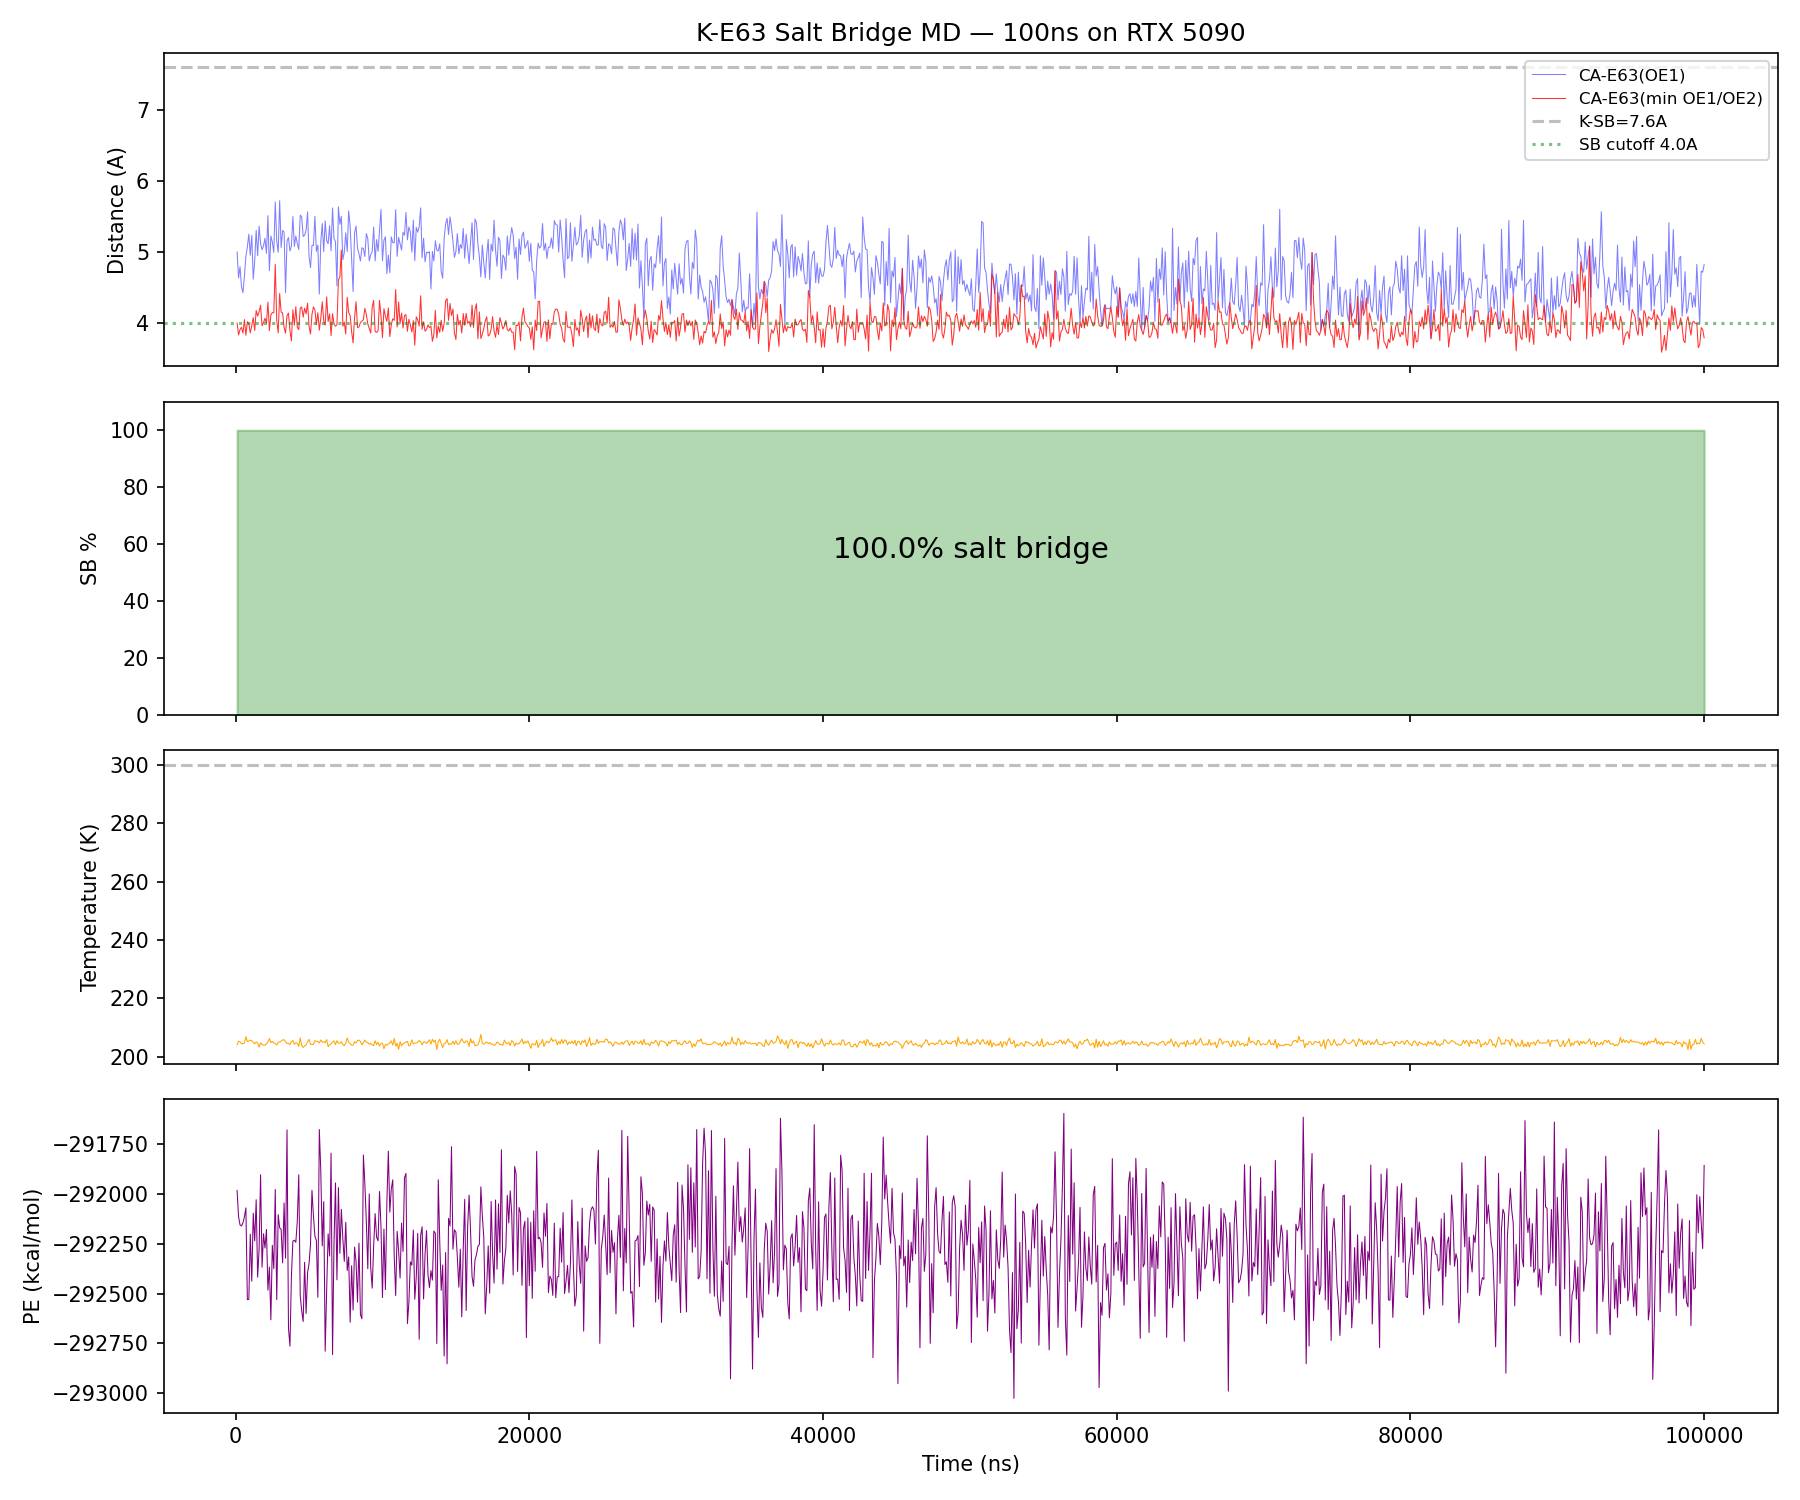
\includegraphics[width=0.9\textwidth]{figures/FigS_MD1_100ns_summary.pdf}
\caption{Fig. S-MD1. 100-ns summary panel (system overview).}
\end{figure}

\begin{figure}[h]
\centering
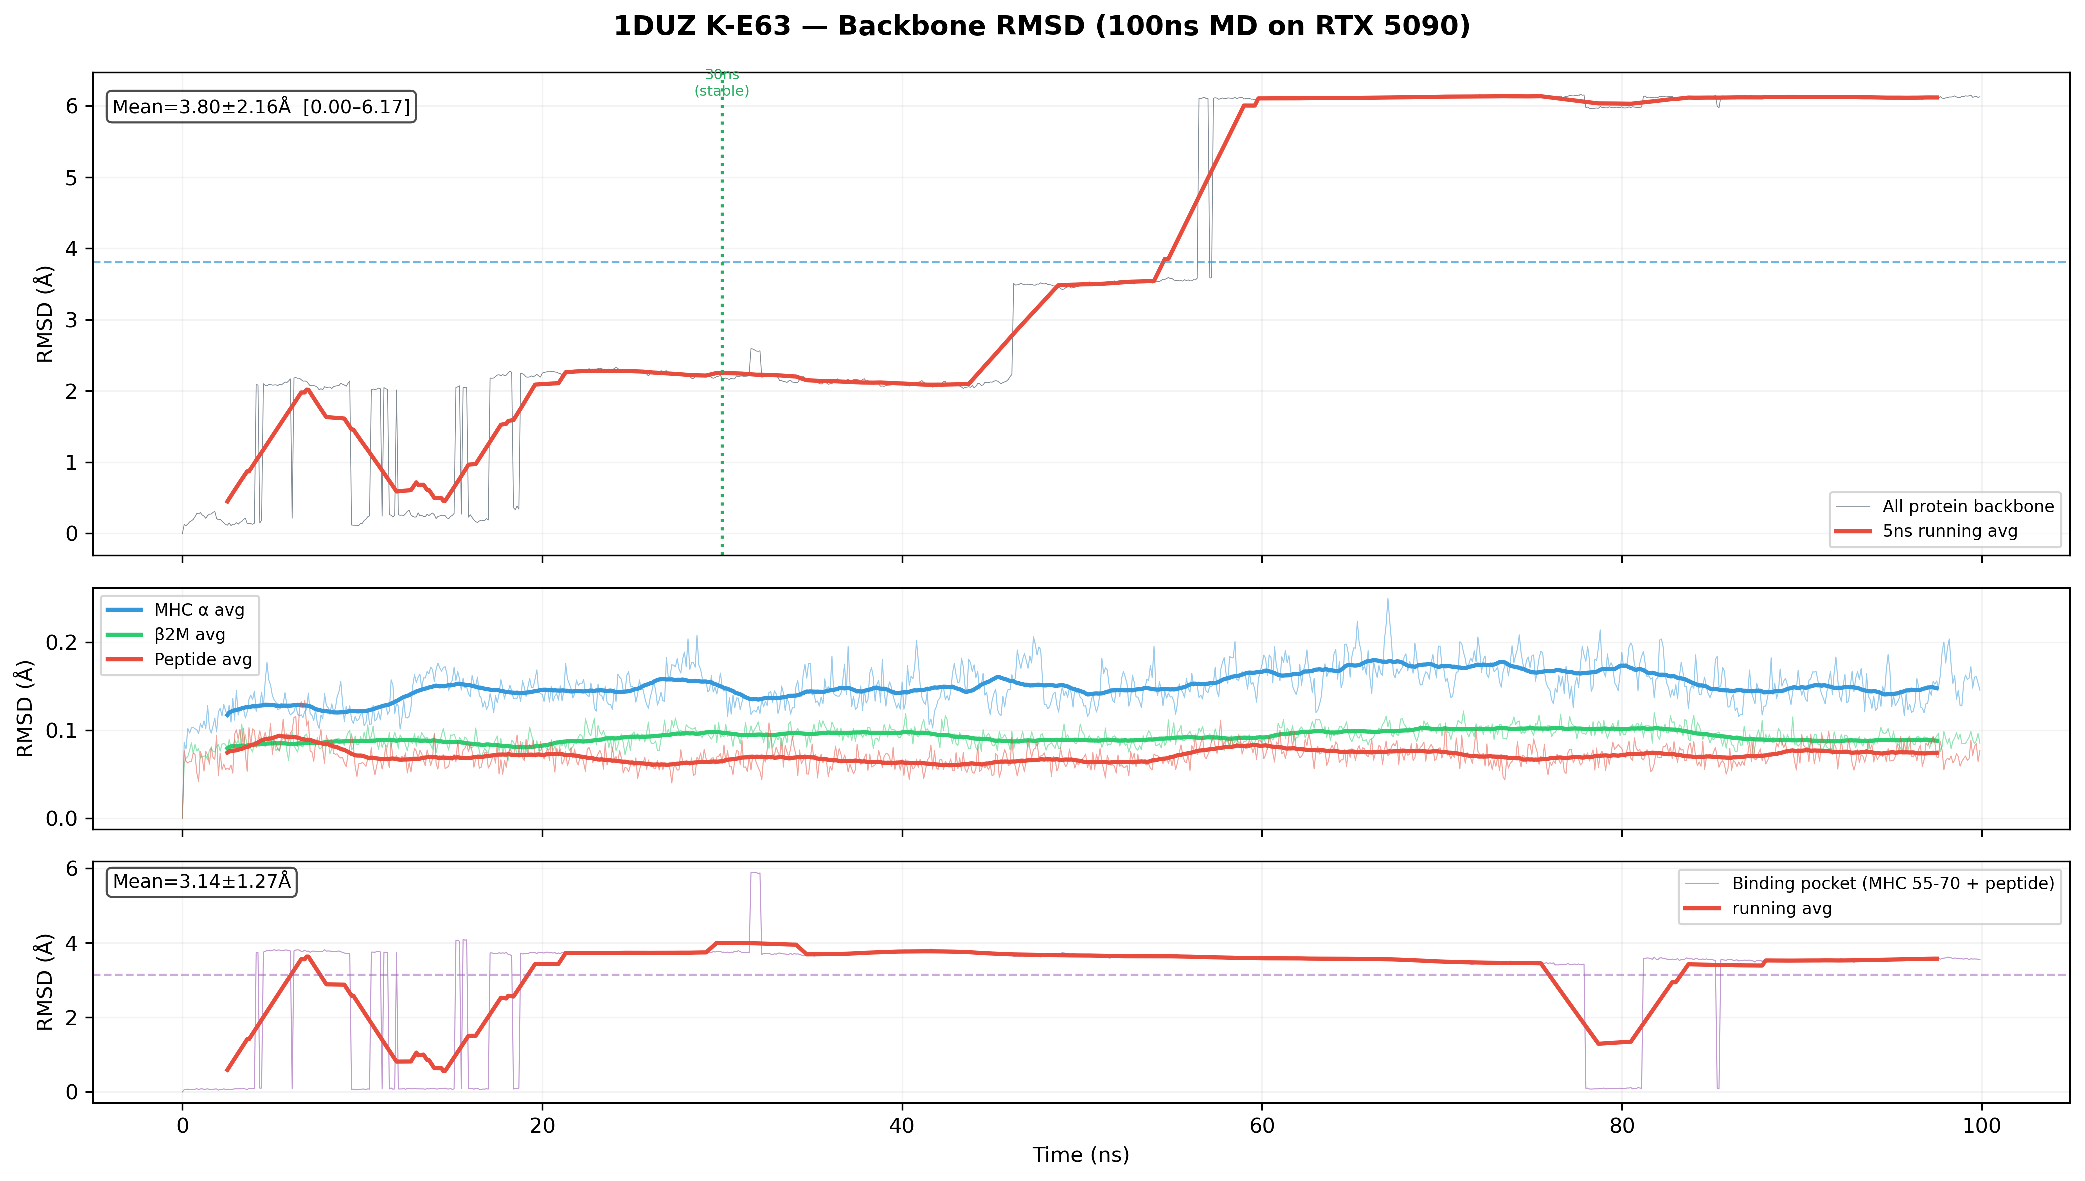
\includegraphics[width=0.9\textwidth]{figures/FigS_MD2_rmsd.pdf}
\caption{Fig. S-MD2. Backbone RMSD over 100 ns (system stability).}
\end{figure}

\begin{figure}[h]
\centering
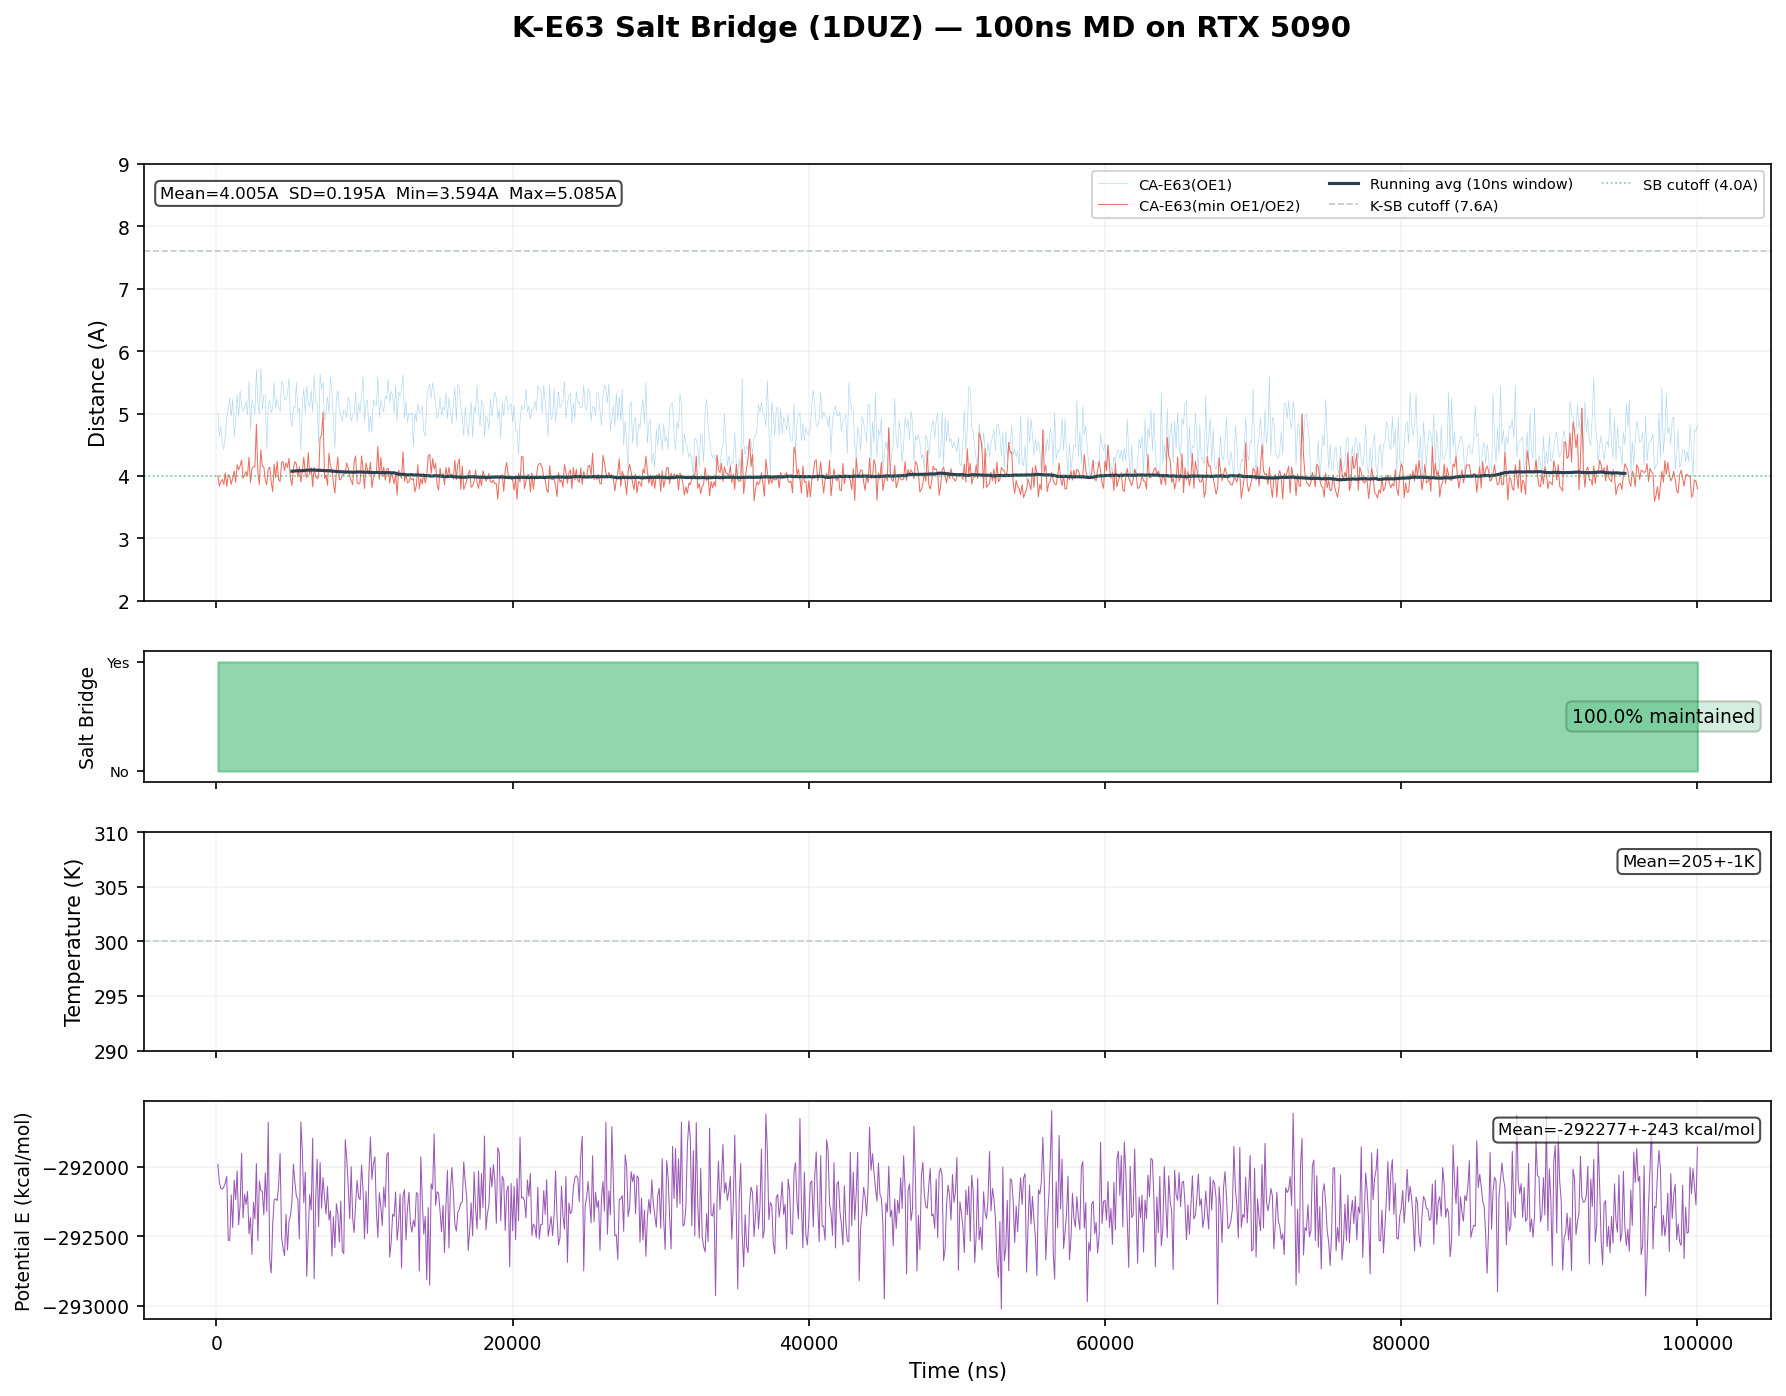
\includegraphics[width=0.9\textwidth]{figures/FigS_MD3_saltbridge_distance.pdf}
\caption{Fig. S-MD3. P2-Lys--Glu63 distance time series (transient salt-bridge contacts).}
\end{figure}

\begin{figure}[h]
\centering
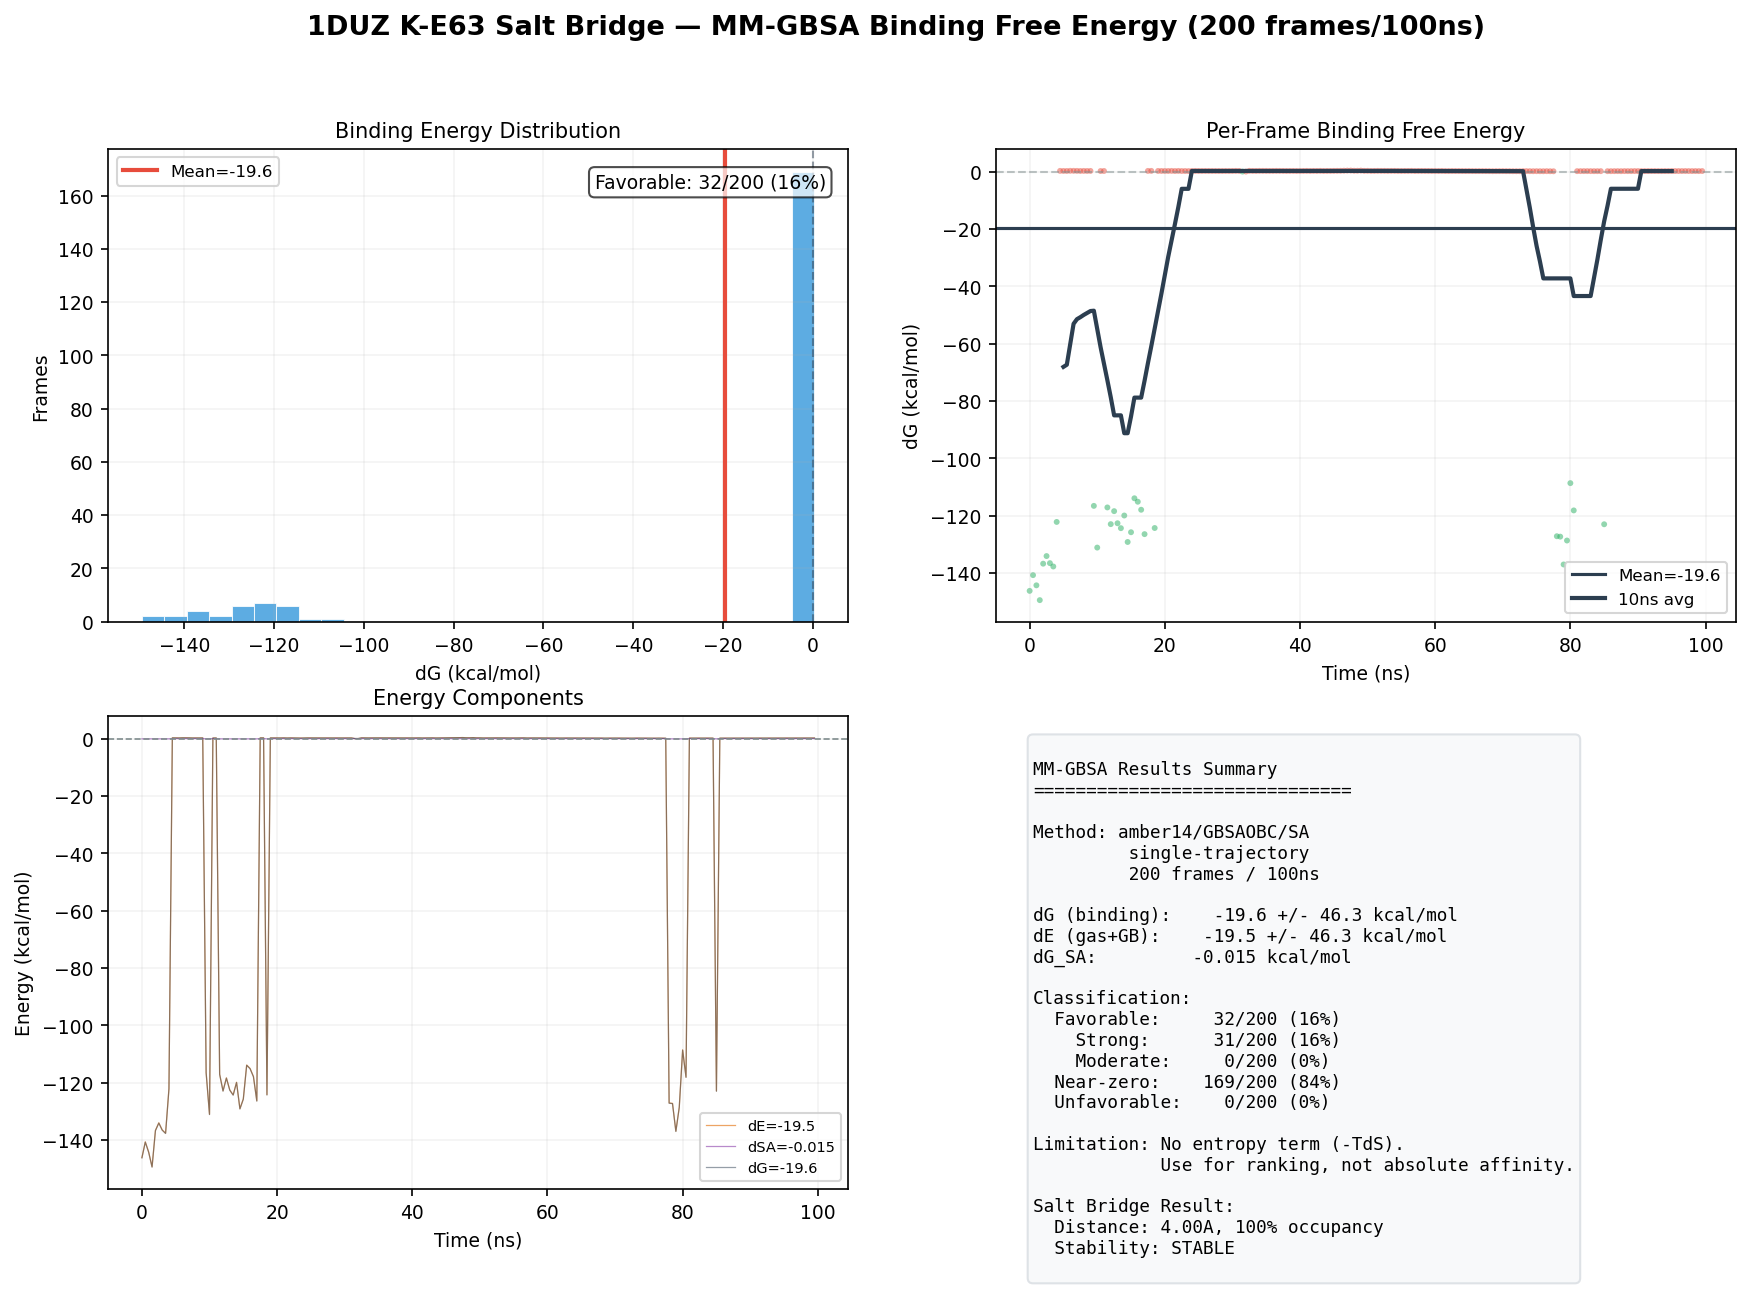
\includegraphics[width=0.9\textwidth]{figures/FigS_MD4_mmgbsa.pdf}
\caption{Fig. S-MD4. MM-GBSA binding-energy distribution.}
\end{figure}

\begin{figure}[h]
\centering
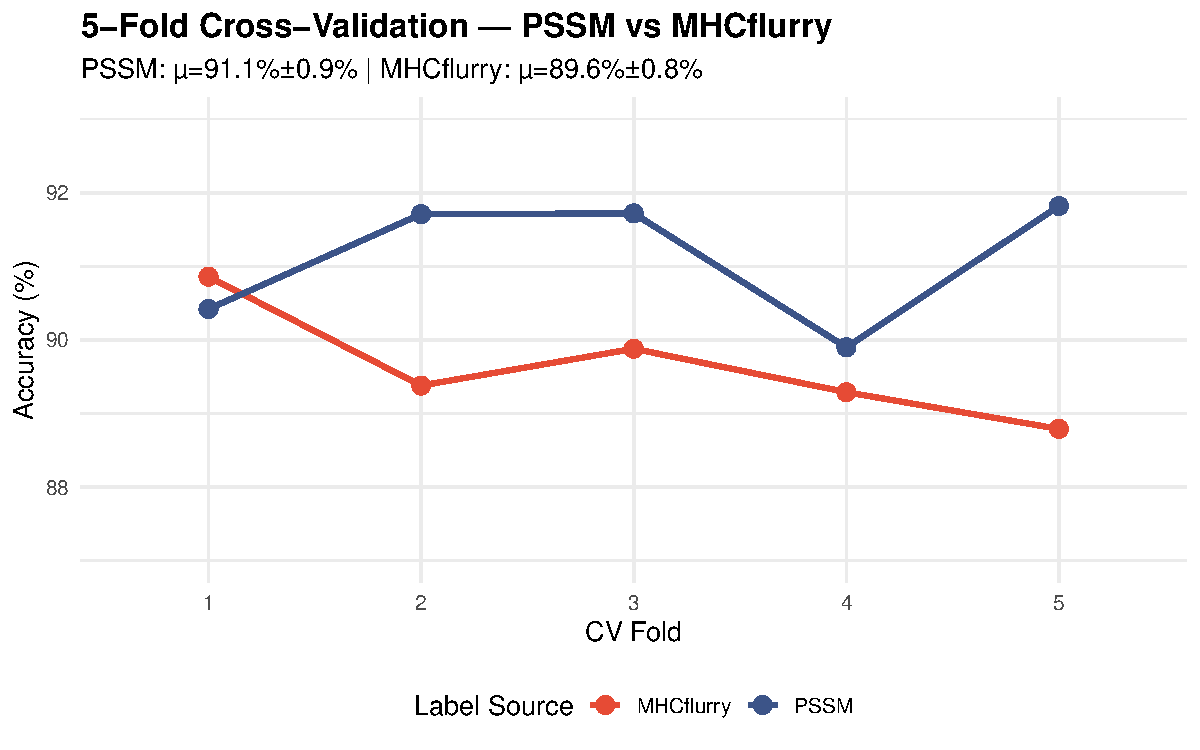
\includegraphics[width=0.9\textwidth]{figures/FigureS1_per_class_f1.pdf}
\caption{Fig. S1. Per-class F1 across architectures.}
\end{figure}

\begin{figure}[h]
\centering
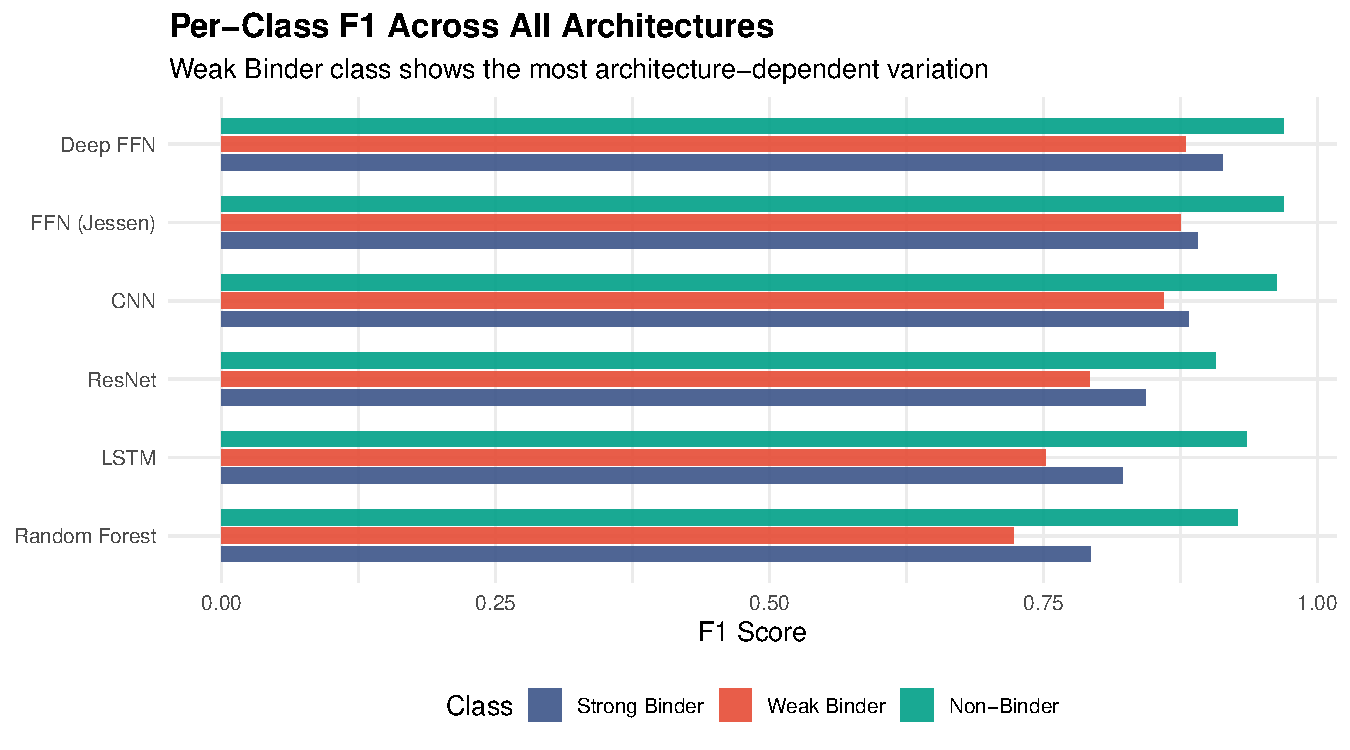
\includegraphics[width=0.9\textwidth]{figures/FigureS2_cv_folds.pdf}
\caption{Fig. S2. Cross-validation folds.}
\end{figure}

\begin{figure}[h]
\centering
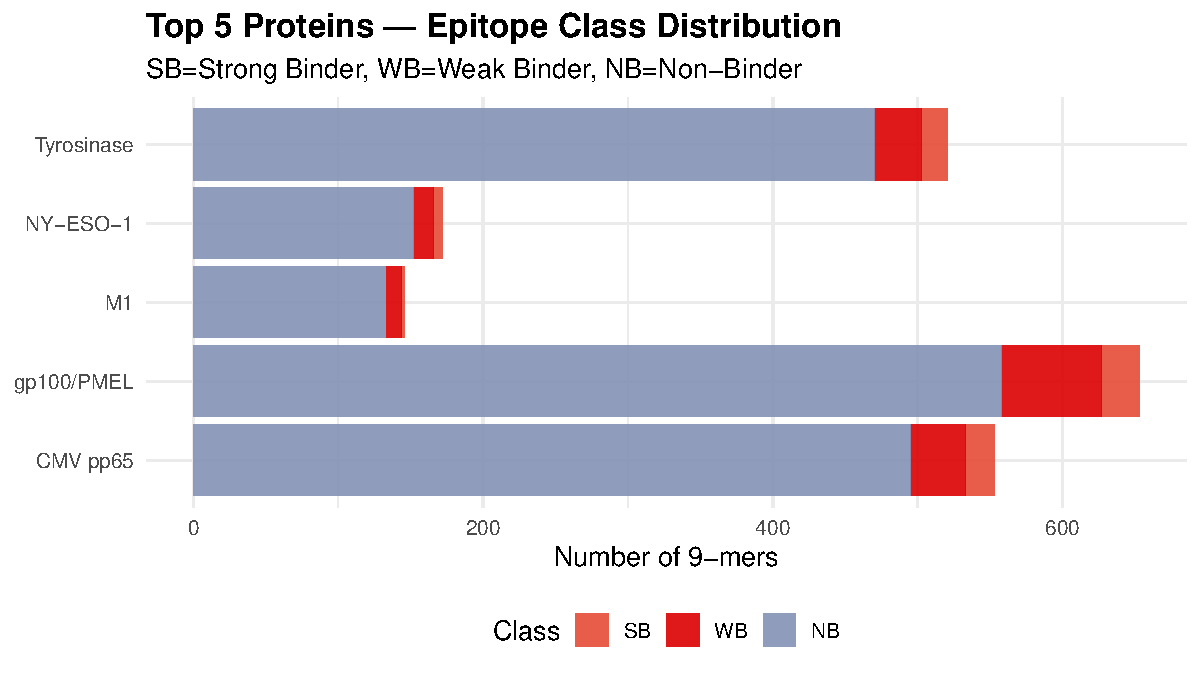
\includegraphics[width=0.9\textwidth]{figures/FigureS3_confusion_matrix.pdf}
\caption{Fig. S3. Confusion matrix.}
\end{figure}

\begin{figure}[h]
\centering
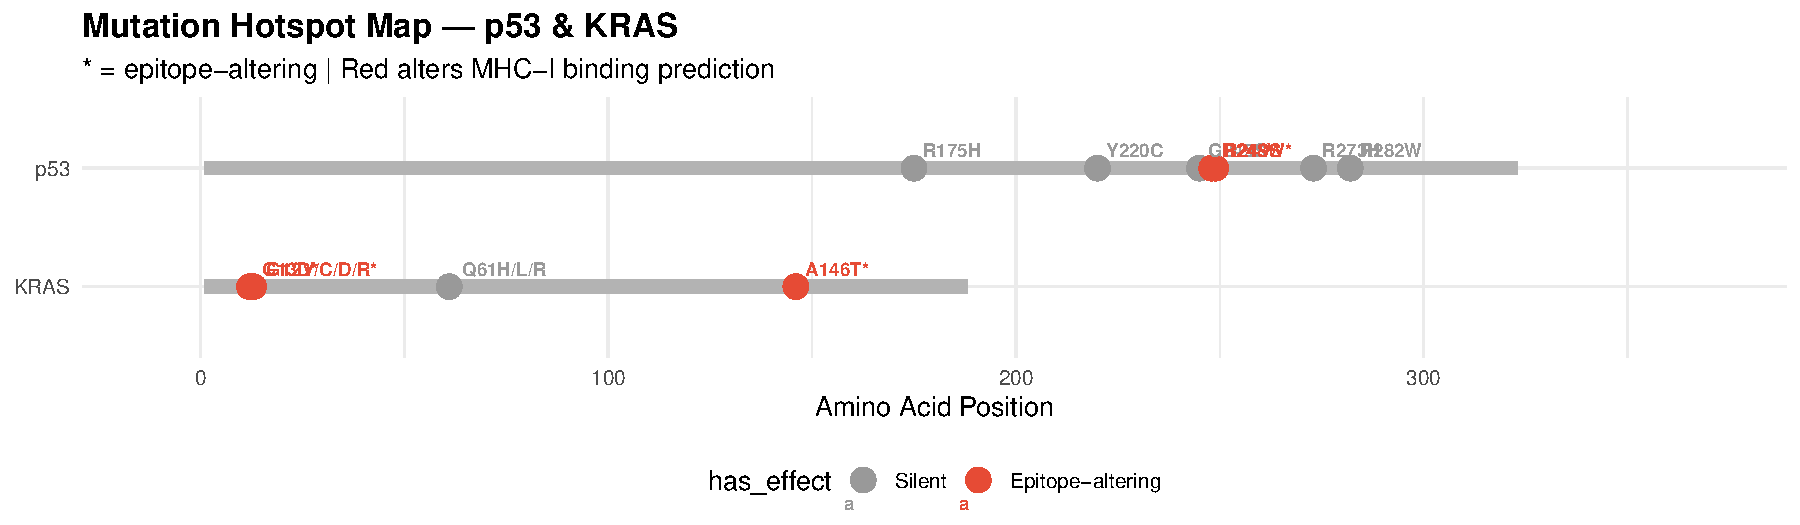
\includegraphics[width=0.9\textwidth]{figures/FigureS4_mutation_paired.pdf}
\caption{Fig. S4. Paired mutation analysis.}
\end{figure}

\begin{figure}[h]
\centering
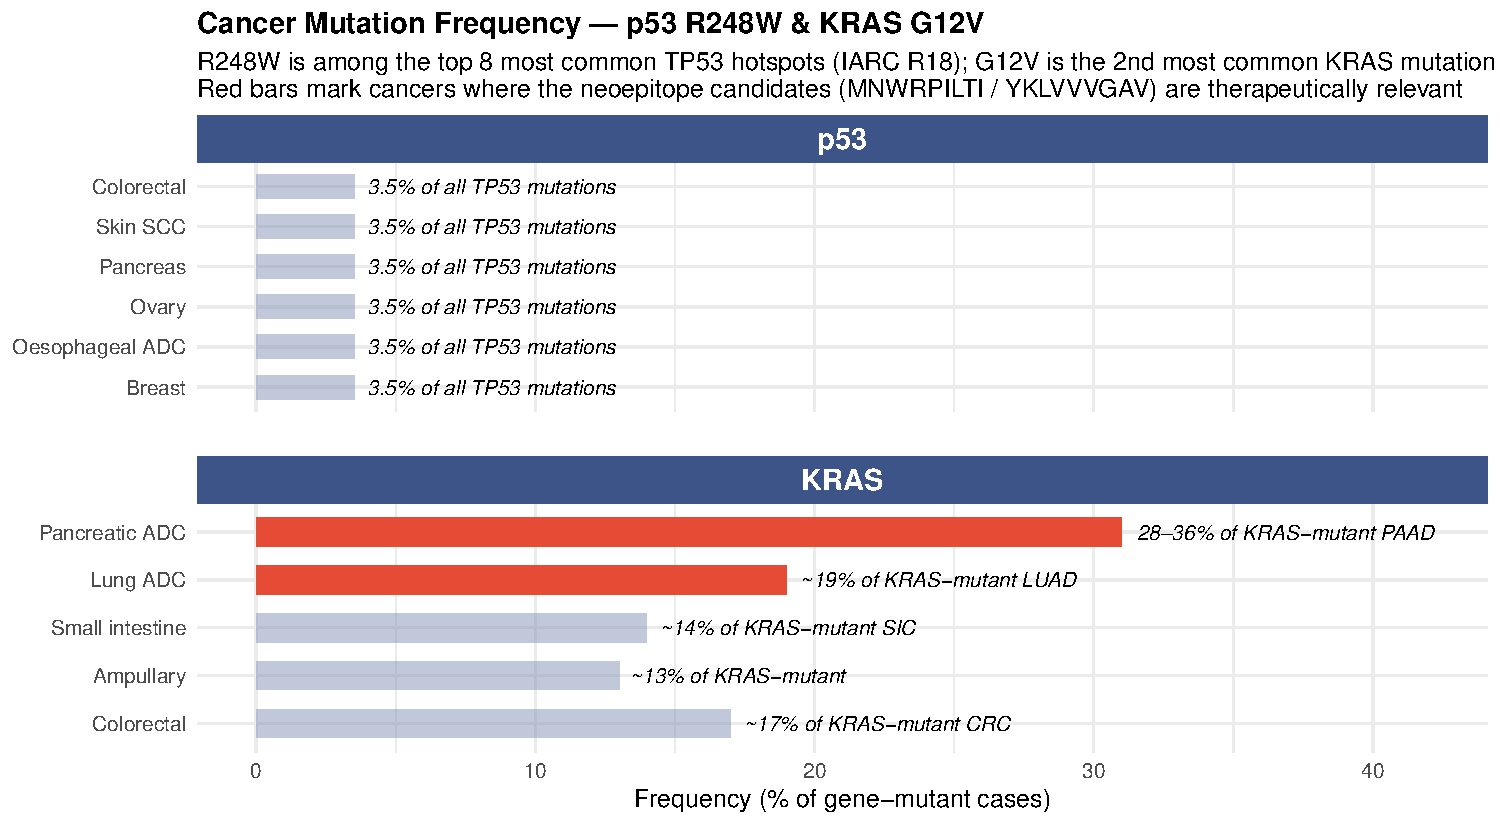
\includegraphics[width=0.9\textwidth]{figures/FigureS5_tcga_frequency.pdf}
\caption{Fig. S5. TCGA mutation frequency.}
\end{figure}

\end{document}
